\documentclass{standalone}
\usepackage[dvipsnames]{xcolor}
\usepackage{pgfplots}
\pgfplotsset{compat=1.18}

\begin{document}

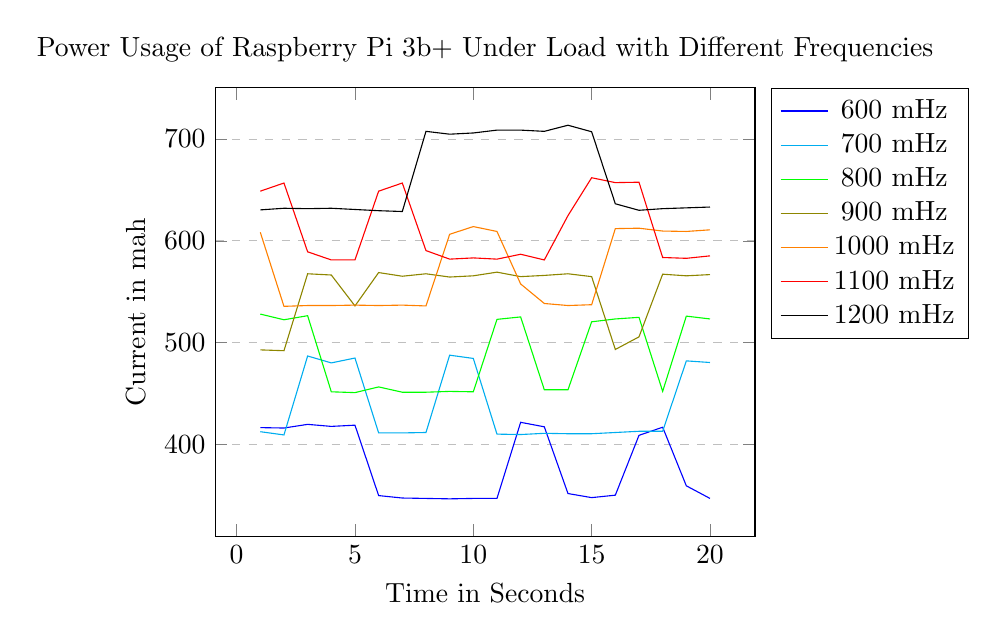
\begin{tikzpicture}
    \begin{axis}[
    title={Power Usage of Raspberry Pi 3b+ Under Load with Different Frequencies},
    xlabel={Time in Seconds},
    ylabel={Current in mah},
    %ytick=data,
    %xtick=data,
    ymajorgrids=true,
    legend pos=outer north east,
    grid style=dashed,
    ]
    \addplot[
        color=blue,
    ]
    coordinates {
        (1,416.40)
        (2,416.00)
        (3,419.60)
        (4,417.60)
        (5,418.80)
        (6,349.60)
        (7,347.20)
        (8,346.80)
        (9,346.40)
        (10,346.80)
        (11,346.80)
        (12,421.60)
        (13,417.20)
        (14,351.60)
        (15,347.60)
        (16,350.00)
        (17,408.80)
        (18,416.80)
        (19,359.20)
        (20,346.80)
    };
    \addlegendentry{600 mHz}
    \addplot[
        color=cyan,
    ]
    coordinates {
        (1,412.40)
        (2,409.20)
        (3,486.80)
        (4,480.00)
        (5,484.80)
        (6,411.20)
        (7,411.20)
        (8,411.60)
        (9,487.60)
        (10,484.40)
        (11,410.00)
        (12,409.60)
        (13,410.80)
        (14,410.40)
        (15,410.40)
        (16,411.60)
        (17,412.80)
        (18,412.80)
        (19,482.00)
        (20,480.40)
    };
    \addlegendentry{700 mHz}
    \addplot[
        color=green,
    ]
    coordinates {
        (1,528.00)
        (2,522.40)
        (3,526.40)
        (4,451.60)
        (5,450.80)
        (6,456.40)
        (7,451.20)
        (8,451.20)
        (9,452.00)
        (10,451.60)
        (11,522.80)
        (12,525.20)
        (13,453.60)
        (14,453.60)
        (15,520.40)
        (16,523.20)
        (17,524.80)
        (18,452.00)
        (19,526.00)
        (20,523.20)
    };
    \addlegendentry{800 mHz}
    \addplot[
        color=olive,
    ]
    coordinates {
        (1,492.80)
        (2,492.00)
        (3,567.60)
        (4,566.40)
        (5,536.00)
        (6,568.80)
        (7,565.20)
        (8,567.60)
        (9,564.40)
        (10,565.60)
        (11,569.20)
        (12,564.80)
        (13,566.00)
        (14,567.60)
        (15,564.80)
        (16,493.20)
        (17,505.60)
        (18,567.20)
        (19,565.60)
        (20,566.80)
    };
    \addlegendentry{900 mHz}
    \addplot[
        color=orange,
    ]
    coordinates {
        (1,608.40)
        (2,535.60)
        (3,536.40)
        (4,536.40)
        (5,536.80)
        (6,536.40)
        (7,536.80)
        (8,536.00)
        (9,606.40)
        (10,614.00)
        (11,609.20)
        (12,557.60)
        (13,538.40)
        (14,536.40)
        (15,537.20)
        (16,612.00)
        (17,612.40)
        (18,609.60)
        (19,609.20)
        (20,610.80)
    };
    \addlegendentry{1000 mHz}
    \addplot[
        color=red,
    ]
    coordinates {
        (1,648.80)
        (2,656.80)
        (3,589.20)
        (4,581.20)
        (5,581.20)
        (6,648.80)
        (7,656.80)
        (8,590.40)
        (9,582.00)
        (10,583.20)
        (11,582.00)
        (12,586.80)
        (13,581.20)
        (14,624.80)
        (15,662.00)
        (16,657.20)
        (17,657.60)
        (18,583.60)
        (19,582.80)
        (20,585.20)
    };
    \addlegendentry{1100 mHz}
    \addplot[
        color=black,
    ]
    coordinates {
        (1,630.40)
        (2,632.00)
        (3,631.60)
        (4,632.00)
        (5,630.80)
        (6,629.60)
        (7,628.80)
        (8,707.60)
        (9,704.80)
        (10,706.00)
        (11,708.80)
        (12,708.80)
        (13,707.60)
        (14,713.60)
        (15,707.20)
        (16,636.40)
        (17,630.00)
        (18,631.60)
        (19,632.40)
        (20,633.20)
    };
    \addlegendentry{1200 mHz}
    \end{axis}
\end{tikzpicture}

\end{document}
